\documentclass[review,12pt]{elsarticle}
\usepackage[T1]{fontenc}
\usepackage[utf8]{inputenc}
\usepackage{newtxtext,newtxmath}
\usepackage{amsmath}
\usepackage{graphicx,booktabs,makecell,multirow,array}
\usepackage[labelfont=bf]{caption}
\usepackage{enumitem}
\usepackage{algorithm}
\usepackage[noend]{algpseudocode}
\usepackage{xcolor}
\usepackage[hidelinks]{hyperref}
\usepackage{lineno}
\linenumbers
\biboptions{numbers,sort&compress}
\journal{Results in Engineering}
\makeatletter
\def\ps@pprintTitle{\let\@oddhead\@empty\let\@evenhead\@empty\let\@oddfoot\@empty\let\@evenfoot\@empty}
\makeatother
% auto-generated by analysis/analyze.py -- do not edit
\newcommand{\RandomReturn}{8.85}
\newcommand{\RandomReturnSD}{2.71}
\newcommand{\RandomOnTimePct}{53.5}
\newcommand{\RandomWOnTimePct}{48.8}
\newcommand{\RandomComplPct}{67.8}
\newcommand{\RandomFatigue}{0.207}
\newcommand{\RandomAttention}{0.855}
\newcommand{\RandomBreakPct}{32.6}
\newcommand{\RandomHighFatPct}{0.0}
\newcommand{\FIFOReturn}{3.49}
\newcommand{\FIFOReturnSD}{3.49}
\newcommand{\FIFOOnTimePct}{43.2}
\newcommand{\FIFOWOnTimePct}{42.2}
\newcommand{\FIFOComplPct}{48.5}
\newcommand{\FIFOFatigue}{0.546}
\newcommand{\FIFOAttention}{0.463}
\newcommand{\FIFOBreakPct}{0.0}
\newcommand{\FIFOHighFatPct}{31.3}
\newcommand{\EDFReturn}{4.24}
\newcommand{\EDFReturnSD}{3.82}
\newcommand{\EDFOnTimePct}{46.8}
\newcommand{\EDFWOnTimePct}{45.4}
\newcommand{\EDFComplPct}{49.1}
\newcommand{\EDFFatigue}{0.545}
\newcommand{\EDFAttention}{0.465}
\newcommand{\EDFBreakPct}{0.0}
\newcommand{\EDFHighFatPct}{30.4}
\newcommand{\SPTReturn}{7.95}
\newcommand{\SPTReturnSD}{2.94}
\newcommand{\SPTOnTimePct}{62.5}
\newcommand{\SPTWOnTimePct}{49.4}
\newcommand{\SPTComplPct}{66.1}
\newcommand{\SPTFatigue}{0.477}
\newcommand{\SPTAttention}{0.543}
\newcommand{\SPTBreakPct}{0.0}
\newcommand{\SPTHighFatPct}{17.3}
\newcommand{\EDFPeriodicReturn}{11.41}
\newcommand{\EDFPeriodicReturnSD}{3.32}
\newcommand{\EDFPeriodicOnTimePct}{66.0}
\newcommand{\EDFPeriodicWOnTimePct}{65.7}
\newcommand{\EDFPeriodicComplPct}{74.1}
\newcommand{\EDFPeriodicFatigue}{0.296}
\newcommand{\EDFPeriodicAttention}{0.798}
\newcommand{\EDFPeriodicBreakPct}{18.8}
\newcommand{\EDFPeriodicHighFatPct}{0.0}
\newcommand{\EDFThresholdReturn}{11.35}
\newcommand{\EDFThresholdReturnSD}{3.28}
\newcommand{\EDFThresholdOnTimePct}{65.4}
\newcommand{\EDFThresholdWOnTimePct}{65.0}
\newcommand{\EDFThresholdComplPct}{74.2}
\newcommand{\EDFThresholdFatigue}{0.288}
\newcommand{\EDFThresholdAttention}{0.806}
\newcommand{\EDFThresholdBreakPct}{20.1}
\newcommand{\EDFThresholdHighFatPct}{0.0}
\newcommand{\CogHeuristicReturn}{10.59}
\newcommand{\CogHeuristicReturnSD}{2.76}
\newcommand{\CogHeuristicOnTimePct}{63.8}
\newcommand{\CogHeuristicWOnTimePct}{53.3}
\newcommand{\CogHeuristicComplPct}{78.0}
\newcommand{\CogHeuristicFatigue}{0.279}
\newcommand{\CogHeuristicAttention}{0.803}
\newcommand{\CogHeuristicBreakPct}{19.8}
\newcommand{\CogHeuristicHighFatPct}{0.0}
\newcommand{\DQNReturn}{10.66}
\newcommand{\DQNReturnSD}{0.33}
\newcommand{\DQNOnTimePct}{68.6}
\newcommand{\DQNWOnTimePct}{60.6}
\newcommand{\DQNComplPct}{73.2}
\newcommand{\DQNFatigue}{0.391}
\newcommand{\DQNAttention}{0.692}
\newcommand{\DQNBreakPct}{10.5}
\newcommand{\DQNHighFatPct}{0.2}
\newcommand{\AADQNReturn}{12.19}
\newcommand{\AADQNReturnSD}{0.27}
\newcommand{\AADQNOnTimePct}{72.6}
\newcommand{\AADQNWOnTimePct}{65.7}
\newcommand{\AADQNComplPct}{76.5}
\newcommand{\AADQNFatigue}{0.326}
\newcommand{\AADQNAttention}{0.761}
\newcommand{\AADQNBreakPct}{15.9}
\newcommand{\AADQNHighFatPct}{0.0}
\newcommand{\bestHeur}{EDF-Periodic}
\newcommand{\bestHeurReturn}{11.41}
\newcommand{\bestHeurOnTimePct}{66.0}
\newcommand{\bestHeurFatigue}{0.296}
\newcommand{\bestHeurBreakPct}{18.8}
\newcommand{\bestHeurAttention}{0.798}
\newcommand{\aaReturn}{12.19}
\newcommand{\aaReturnSD}{0.27}
\newcommand{\aaOnTimePct}{72.6}
\newcommand{\aaFatigue}{0.326}
\newcommand{\edfOnTimePct}{46.8}
\newcommand{\edfFatigue}{0.545}
\newcommand{\fatigueRedVsEdfPct}{40}
\newcommand{\onTimeGainVsEdfPP}{25.8}
\newcommand{\dRetRandom}{3.34}
\newcommand{\dRetRandomLo}{3.13}
\newcommand{\dRetRandomHi}{3.55}
\newcommand{\rbRetRandom}{0.97}
\newcommand{\winRetRandomPct}{92.8}
\newcommand{\seedsRetRandom}{10}
\newcommand{\dRetFIFO}{8.70}
\newcommand{\dRetFIFOLo}{8.47}
\newcommand{\dRetFIFOHi}{8.92}
\newcommand{\rbRetFIFO}{1.00}
\newcommand{\winRetFIFOPct}{99.8}
\newcommand{\seedsRetFIFO}{10}
\newcommand{\dRetEDF}{7.95}
\newcommand{\dRetEDFLo}{7.71}
\newcommand{\dRetEDFHi}{8.18}
\newcommand{\rbRetEDF}{1.00}
\newcommand{\winRetEDFPct}{100.0}
\newcommand{\seedsRetEDF}{10}
\newcommand{\dRetSPT}{4.24}
\newcommand{\dRetSPTLo}{4.06}
\newcommand{\dRetSPTHi}{4.41}
\newcommand{\rbRetSPT}{1.00}
\newcommand{\winRetSPTPct}{99.0}
\newcommand{\seedsRetSPT}{10}
\newcommand{\dRetEDFPeriodic}{0.77}
\newcommand{\dRetEDFPeriodicLo}{0.58}
\newcommand{\dRetEDFPeriodicHi}{0.95}
\newcommand{\rbRetEDFPeriodic}{0.34}
\newcommand{\winRetEDFPeriodicPct}{58.6}
\newcommand{\seedsRetEDFPeriodic}{10}
\newcommand{\dRetEDFThreshold}{0.84}
\newcommand{\dRetEDFThresholdLo}{0.66}
\newcommand{\dRetEDFThresholdHi}{1.02}
\newcommand{\rbRetEDFThreshold}{0.37}
\newcommand{\winRetEDFThresholdPct}{60.4}
\newcommand{\seedsRetEDFThreshold}{10}
\newcommand{\dRetCogHeuristic}{1.59}
\newcommand{\dRetCogHeuristicLo}{1.45}
\newcommand{\dRetCogHeuristicHi}{1.74}
\newcommand{\rbRetCogHeuristic}{0.83}
\newcommand{\winRetCogHeuristicPct}{81.6}
\newcommand{\seedsRetCogHeuristic}{10}
\newcommand{\dOnRandom}{19.1}
\newcommand{\dOnRandomLo}{18.2}
\newcommand{\dOnRandomHi}{20.2}
\newcommand{\rbOnRandom}{1.00}
\newcommand{\winOnRandomPct}{95.8}
\newcommand{\seedsOnRandom}{10}
\newcommand{\dOnFIFO}{29.4}
\newcommand{\dOnFIFOLo}{28.6}
\newcommand{\dOnFIFOHi}{30.3}
\newcommand{\rbOnFIFO}{1.00}
\newcommand{\winOnFIFOPct}{99.0}
\newcommand{\seedsOnFIFO}{10}
\newcommand{\dOnEDF}{25.8}
\newcommand{\dOnEDFLo}{24.9}
\newcommand{\dOnEDFHi}{26.7}
\newcommand{\rbOnEDF}{1.00}
\newcommand{\winOnEDFPct}{99.0}
\newcommand{\seedsOnEDF}{10}
\newcommand{\dOnSPT}{10.1}
\newcommand{\dOnSPTLo}{9.4}
\newcommand{\dOnSPTHi}{10.8}
\newcommand{\rbOnSPT}{0.93}
\newcommand{\winOnSPTPct}{88.2}
\newcommand{\seedsOnSPT}{10}
\newcommand{\dOnEDFPeriodic}{6.6}
\newcommand{\dOnEDFPeriodicLo}{5.7}
\newcommand{\dOnEDFPeriodicHi}{7.5}
\newcommand{\rbOnEDFPeriodic}{0.67}
\newcommand{\winOnEDFPeriodicPct}{67.0}
\newcommand{\seedsOnEDFPeriodic}{10}
\newcommand{\dOnEDFThreshold}{7.3}
\newcommand{\dOnEDFThresholdLo}{6.4}
\newcommand{\dOnEDFThresholdHi}{8.2}
\newcommand{\rbOnEDFThreshold}{0.71}
\newcommand{\winOnEDFThresholdPct}{68.0}
\newcommand{\seedsOnEDFThreshold}{10}
\newcommand{\dOnCogHeuristic}{8.8}
\newcommand{\dOnCogHeuristicLo}{8.2}
\newcommand{\dOnCogHeuristicHi}{9.4}
\newcommand{\rbOnCogHeuristic}{0.93}
\newcommand{\winOnCogHeuristicPct}{84.6}
\newcommand{\seedsOnCogHeuristic}{10}
\newcommand{\dFatRandom}{0.119}
\newcommand{\dFatRandomLo}{0.115}
\newcommand{\dFatRandomHi}{0.124}
\newcommand{\rbFatRandom}{1.00}
\newcommand{\winFatRandomPct}{98.8}
\newcommand{\seedsFatRandom}{10}
\newcommand{\dFatFIFO}{-0.220}
\newcommand{\dFatFIFOLo}{-0.225}
\newcommand{\dFatFIFOHi}{-0.215}
\newcommand{\rbFatFIFO}{-1.00}
\newcommand{\winFatFIFOPct}{0.0}
\newcommand{\seedsFatFIFO}{0}
\newcommand{\dFatEDF}{-0.219}
\newcommand{\dFatEDFLo}{-0.223}
\newcommand{\dFatEDFHi}{-0.214}
\newcommand{\rbFatEDF}{-1.00}
\newcommand{\winFatEDFPct}{0.0}
\newcommand{\seedsFatEDF}{0}
\newcommand{\dFatSPT}{-0.151}
\newcommand{\dFatSPTLo}{-0.155}
\newcommand{\dFatSPTHi}{-0.147}
\newcommand{\rbFatSPT}{-1.00}
\newcommand{\winFatSPTPct}{0.0}
\newcommand{\seedsFatSPT}{0}
\newcommand{\dFatEDFPeriodic}{0.030}
\newcommand{\dFatEDFPeriodicLo}{0.026}
\newcommand{\dFatEDFPeriodicHi}{0.033}
\newcommand{\rbFatEDFPeriodic}{0.68}
\newcommand{\winFatEDFPeriodicPct}{77.6}
\newcommand{\seedsFatEDFPeriodic}{10}
\newcommand{\dFatEDFThreshold}{0.038}
\newcommand{\dFatEDFThresholdLo}{0.036}
\newcommand{\dFatEDFThresholdHi}{0.041}
\newcommand{\rbFatEDFThreshold}{0.92}
\newcommand{\winFatEDFThresholdPct}{91.0}
\newcommand{\seedsFatEDFThreshold}{10}
\newcommand{\dFatCogHeuristic}{0.047}
\newcommand{\dFatCogHeuristicLo}{0.044}
\newcommand{\dFatCogHeuristicHi}{0.049}
\newcommand{\rbFatCogHeuristic}{0.98}
\newcommand{\winFatCogHeuristicPct}{94.8}
\newcommand{\seedsFatCogHeuristic}{10}
\newcommand{\dRetVsDqn}{1.53}
\newcommand{\dRetVsDqnLo}{1.46}
\newcommand{\dRetVsDqnHi}{1.60}
\newcommand{\winRetVsDqnPct}{98.4}
\newcommand{\ablFullDiff}{0.77}
\newcommand{\ablFullLo}{0.58}
\newcommand{\ablFullHi}{0.96}
\newcommand{\ablFullDiffOnPP}{6.6}
\newcommand{\ablFullDiffOnLo}{5.7}
\newcommand{\ablFullDiffOnHi}{7.5}
\newcommand{\ablFullRet}{12.19}
\newcommand{\ablFullOnPct}{72.6}
\newcommand{\ablFullBest}{EDF-Periodic}
\newcommand{\ablFullBestRet}{11.41}
\newcommand{\ablFullBestOnPct}{66.0}
\newcommand{\ablFullP}{<10^{-4}}
\newcommand{\ablFullPOn}{<10^{-4}}
\newcommand{\ablFullFatigue}{0.326}
\newcommand{\trainTimeAA}{474}
\newcommand{\trainTimeDQN}{410}
\newcommand{\inferUs}{101}
\newcommand{\DQNSelReturn}{10.66}
\newcommand{\DQNSelOnTimePct}{68.6}
\newcommand{\DQNBestEp}{950}
\newcommand{\DQNFinalReturn}{9.47}
\newcommand{\DQNFinalOnTimePct}{64.8}
\newcommand{\AADQNSelReturn}{12.19}
\newcommand{\AADQNSelOnTimePct}{72.6}
\newcommand{\AADQNBestEp}{1480}
\newcommand{\AADQNFinalReturn}{11.35}
\newcommand{\AADQNFinalOnTimePct}{70.6}


\begin{document}
\begin{frontmatter}
\title{Attention-aware task scheduling under partial observability of human cognitive state: a memory-augmented deep reinforcement learning approach}

\author[vit]{P.\,N. Bhargav Teja}
\author[vit]{Lanka Sree Chathurya}
\author[vit]{Rajay Vedaraj I.S.\corref{cor1}}
\ead{rajay@vit.ac.in}
\cortext[cor1]{Corresponding author.}
\affiliation[vit]{organization={Vellore Institute of Technology},
            city={Vellore},
            postcode={632014},
            state={Tamil Nadu},
            country={India}}

\begin{abstract}
Dispatching rules such as earliest-deadline-first (EDF) and shortest-processing-time (SPT) assume constant processing capacity, which fails when the resource is a person whose attention depletes, whose fatigue accumulates and whose alertness follows a circadian rhythm. We formulate human-centric task scheduling as a partially observable Markov decision process in which rest is an explicit action, attention and fatigue are latent states observed through noisy estimates, and a multi-objective reward balances deadline-weighted task value against cognitive load. We propose an attention-aware deep Q-network (AA-DQN) that combines an observation history, as an approximation of the belief state, with Double Q-learning and a dueling architecture. In a cognitively grounded simulator, AA-DQN was benchmarked against nine rule-based schedulers, including grid-tuned EDF and SPT rules with periodic or state-triggered rest, using ten training seeds, 500 held-out workdays with common random numbers and multiplicity-corrected tests. Rules that never rest performed poorly (EDF: \edfOnTimePct\% of tasks on time). The pre-specified AA-DQN matched the return of the best tuned rule and completed more tasks on time (\aaOnTimePct\% versus \bestHeurOnTimePct\%). A compact variant with intensity-only actions, evaluated as a secondary analysis, exceeded the best rule in return (+\SecRetSPTThreshold, $p<0.001$) and on-time completion (\AADQNThreeactOnTimePct\%). The learned policies alone combined high throughput with protection of demanding tasks: they front-load hard work while attention is high and rest around the post-lunch dip. Their advantage grew markedly with accurate cognitive-state estimates, and they were robust to sensor noise, whereas generalisation to unseen workloads remained limited.
\end{abstract}

\begin{keyword}
Human-centric scheduling \sep Deep reinforcement learning \sep Partially observable Markov decision process \sep Cognitive fatigue \sep Attention \sep Rest-break scheduling \sep Industry 5.0
\end{keyword}

\end{frontmatter}

\section{Introduction}\label{sec:intro}

Scheduling decides which piece of work is executed when, and it is one of the oldest problems in operations research and computer engineering \cite{smith1956,jackson1955,graham1979,pinedo2016}. Classical dispatching rules such as First-In-First-Out (FIFO), Shortest Processing Time (SPT) and Earliest Deadline First (EDF) are attractive because they are transparent, cheap to compute and, under the right assumptions, provably optimal: EDF minimises maximum lateness on a single resource with constant capacity \cite{jackson1955,liu1973}, and SPT minimises mean flow time \cite{smith1956}. The common assumption underlying these guarantees is that the resource executing the work has a \emph{fixed, state-independent processing capacity}. This assumption is reasonable for processors and machines but is violated whenever the resource is a person.

Human work capacity is dynamic. Sustained effort depletes attentional resources and produces the vigilance decrement first documented by Mackworth~\cite{mackworth1948} and since replicated across many tasks \cite{warm2008,thomson2015,esterman2019}; mental fatigue accumulates with time-on-task and degrades both speed and accuracy \cite{boksem2008,lorist2000,hockey2013,ackerman2011}; and alertness follows a circadian rhythm with a pronounced early-afternoon dip \cite{akerstedt1997,monk2005,schmidt2007,blatter2007}. Rest breaks partially reverse these effects, and field studies consistently report that well-timed breaks preserve or even increase productivity despite the time they consume \cite{henning1997,dababneh2001,galinsky2000,tucker2003,albulescu2022}. A schedule that is optimal for a constant-capacity machine can therefore be poor for a human: it front-loads demanding work regardless of cognitive state, never allocates recovery, and drives the worker into a low-capacity regime in which deadlines are missed precisely because capacity was ignored. The concern is not only productivity. Chronic fatigue is associated with errors and accidents \cite{dawson1997,williamson2011}, and the move from Industry~4.0 towards a human-centric Industry~5.0 explicitly calls for production and service systems that adapt to the well-being of their workers rather than the reverse \cite{breque2021,xu2021,lu2022,leng2022,ivanov2023}.

Operations-management research has long recognised this gap. Models of worker fatigue and recovery have been integrated into dual-resource-constrained systems \cite{jaber2010,jaber2013,givi2015}, rest-allowance and break-scheduling problems have been formulated analytically \cite{bechtold1984,konz1998,calzavara2019}, and taxonomies for merging scheduling theory with human factors have been proposed \cite{lodree2009,neumann2010,boudreau2003,katiraee2021}. These approaches, however, usually assume that the worker's state is known or deterministic and optimise an offline plan; they do not provide an adaptive \emph{policy} that reacts to the evolving, uncertain state of a specific person during the day. Deep reinforcement learning (DRL), in turn, has produced effective adaptive schedulers for job shops, clusters and production lines \cite{mao2016,mao2019,waschneck2018,luo2020,zhang2020l2d,park2021,song2023}, and recent surveys document rapid growth of the field \cite{kayhan2023,panzer2022,khadivi2025}. Yet the resources in these studies are machines, and the few recent studies that include worker fatigue embed it in large shop-floor models where fatigue is a deterministic, fully observed variable \cite{tan2021,hu2025}. Two features of the human problem are thus rarely addressed together: \emph{the decision of when to rest is itself a scheduling action}, and \emph{the cognitive state that should drive that decision cannot be measured directly}. In practice, attention and fatigue are inferred from noisy proxies such as physiological signals, eye tracking, performance probes or self-report \cite{charles2019,borghini2014,hogervorst2014,basner2011,hart1988}, which makes the scheduling problem partially observable.

This paper studies attention-aware task scheduling for a single knowledge or production worker as a partially observable Markov decision process (POMDP) \cite{astrom1965,smallwood1973,kaelbling1998} and solves it with a memory-augmented deep Q-network. We pay particular attention to the methodological issues that make DRL comparisons hard to trust \cite{henderson2018,agarwal2021}: we compare against strong, \emph{tuned}, cognition-aware heuristics rather than only against FIFO and EDF; we use disjoint seed sets for training, tuning and testing; we evaluate on 500 held-out workdays with common random numbers; we report ten independent training seeds with confidence intervals and multiplicity-corrected paired tests; and we separate effects of the reward function from effects of the dynamics through ablation.

The contributions are as follows.
\begin{enumerate}[label=(\roman*)]
  \item \textbf{A cognitively grounded scheduling simulator.} We formulate a workday-scale scheduling environment in which a latent homeostatic attention resource, an exponentially accumulating and recovering fatigue state \cite{jaber2010}, and a circadian process \cite{akerstedt1997,monk2005} jointly determine the worker's instantaneous work rate. Tasks arrive stochastically with heterogeneous difficulty, work content and deadlines. Rest is an explicit action. The simulator, its parameters and their behavioural rationale are fully specified and released.
  \item \textbf{A POMDP formulation with a multi-objective reward.} The scheduler observes only noisy estimates of attention and fatigue together with a compact, size-invariant summary of the task queue. The reward combines deadline-weighted task value with explicit attention and fatigue terms, and we analyse the resulting productivity--fatigue trade-off as a Pareto front \cite{roijers2013,hayes2022}.
  \item \textbf{An attention-aware DQN (AA-DQN).} We combine a finite observation history, which acts as an approximate sufficient statistic for the belief state \cite{singh1994,hausknecht2015,ni2022}, with Double Q-learning \cite{vanhasselt2016} and a dueling architecture \cite{wang2016dueling}. A component ablation quantifies the contribution of each element.
  \item \textbf{A rigorous empirical study.} Against seven baselines, including grid-tuned threshold and attention-matching heuristics that observe the same noisy cognitive signals, we test (a) whether learning helps, (b) \emph{why} it helps, through environment ablations that remove observation noise, the circadian process, the cognitive dynamics or the cognitive reward terms, (c) what behaviour is learned, and (d) how the learned policy generalises to unseen worker profiles, workloads and sensor-noise levels.
\end{enumerate}

The remainder of the paper is organised as follows. Section~\ref{sec:related} reviews related work and positions the study. Section~\ref{sec:problem} formulates the problem. Section~\ref{sec:method} presents AA-DQN. Section~\ref{sec:setup} details the experimental protocol. Section~\ref{sec:results} reports results, Section~\ref{sec:discussion} discusses implications, ethics and limitations, and Section~\ref{sec:conclusion} concludes.

\section{Related work}\label{sec:related}

\subsection{Classical and dynamic scheduling}
Single-resource sequencing theory provides the canonical dispatching rules and their optimality conditions: SPT for mean flow time \cite{smith1956}, EDF for maximum lateness \cite{jackson1955}, and the Moore--Hodgson algorithm for the number of late jobs \cite{moore1968}. The three-field classification of \citet{graham1979} and the textbook treatment of \citet{pinedo2016} organise the deterministic theory. In real-time computing, EDF is optimal for preemptive scheduling of independent tasks whenever the processor is not overloaded \cite{liu1973}, but its performance can collapse under overload, when a domino effect causes many deadlines to be missed \cite{buttazzo2011}. This failure mode is directly relevant here, because a fatigued worker is in effect an overloaded resource. Surveys of priority rules \cite{panwalkar1977,haupt1989} and of dynamic and reactive scheduling \cite{vieira2003,ouelhadj2009} show that practice relies heavily on such rules when information arrives online. In all of these models, however, processing times are exogenous: they do not depend on the history of the schedule.

\subsection{Human factors in scheduling and workforce models}
Personnel scheduling and rostering \cite{ernst2004,burke2004,vandenbergh2013} assign workers to shifts but typically treat performance within a shift as constant. Research at the interface of operations and human resources argues that this abstraction misses first-order effects \cite{boudreau2003,neumann2010}, and \citet{lodree2009} proposed a taxonomy for integrating human factors into scheduling theory. Quantitative models of learning, forgetting, fatigue and recovery have been developed for dual-resource-constrained systems \cite{wright1936,jaber2010,jaber2013,givi2015}. They use exponential fatigue accumulation during work and exponential recovery during rest, which is the functional form we adopt. Rest-break scheduling has been formulated as an optimisation problem since \citet{bechtold1984}, with ergonomic guidance on work--rest ratios summarised by \citet{konz1998} and rest-allowance models for task assignment developed by \citet{calzavara2019}. Fatigue has also been incorporated into flexible job-shop formulations solved by metaheuristics \cite{tan2021} and, very recently, by graph-based DRL \cite{hu2025}. Reviews of human factors in Industry~4.0 and in order picking \cite{grosse2017,kadir2019,neumann2021,katiraee2021} conclude that worker heterogeneity and well-being are still under-represented in operational models. A common feature of this literature is that the worker state is assumed to be known, either deterministic or computed from the schedule, so the decision problem is fully observable.

\subsection{Deep reinforcement learning for scheduling}
Reinforcement learning has been applied to scheduling since the mid-1990s \cite{zhang1995,aydin2000}, and the combination of Q-learning \cite{watkins1992} with deep function approximation \cite{mnih2015} enabled scheduling policies that operate on rich state representations. Notable examples include cluster resource management \cite{mao2016}, data-processing job scheduling with graph neural networks \cite{mao2019}, semiconductor production scheduling \cite{waschneck2018}, dynamic flexible job shops with job insertions \cite{luo2020,song2023}, and size-agnostic job-shop dispatching \cite{zhang2020l2d,park2021,liu2020}. Parameter-adaptive RL for dynamic job shops \cite{shahrabi2017} and RL for combinatorial optimisation more broadly \cite{bengio2021,mazyavkina2021} complete the picture. Systematic reviews \cite{kayhan2023,panzer2022,khadivi2025} note three recurring weaknesses: comparisons against untuned or weak baselines, limited statistical analysis, and little attention to human resources. Our study addresses all three.

\subsection{Cognitive state, its measurement, and adaptive systems}
Resource theories of attention \cite{kahneman1973,wickens2008} and cognitive load theory \cite{sweller1988} model mental capacity as a limited resource. Vigilance research shows that this resource is depleted by sustained effort \cite{mackworth1948,warm2008} and partially restored by brief breaks \cite{ariga2011}. Accounts of fatigue as an effort-regulation or opportunity-cost signal \cite{hockey2013,kurzban2013} and evidence linking fatigue to disengagement \cite{hopstaken2015} motivate treating fatigue as a state variable that shapes future capacity. Biomathematical fatigue models, from the two-process model of sleep regulation \cite{borbely1982,daan1984,borbely2016} to the three-process model of alertness \cite{akerstedt1997} and applied models such as SAFTE \cite{hursh2004}, combine homeostatic and circadian components. We borrow this decomposition at the time scale of a single workday. Recovery research in organisational psychology confirms the value of micro-breaks \cite{sonnentag2007,fritz2013,kim2017,albulescu2022}. On the measurement side, workload and fatigue can be estimated from EEG, cardiac, ocular and behavioural signals \cite{gevins2003,borghini2014,hogervorst2014,charles2019,shaffer2017}, from vigilance probes such as the PVT \cite{dinges1985,basner2011}, or from questionnaires such as NASA-TLX \cite{hart1988,young2015}. All of these estimates are noisy. Adaptive automation and physiological computing use such estimates to adjust system behaviour \cite{byrne1996,parasuraman2000,kaber2004,fairclough2009,zander2011,feigh2012}, and interruption-management systems decide when to notify a user based on inferred cognitive state \cite{horvitz2003,iqbal2008,czerwinski2004,mark2008}. Reinforcement learning has been used to personalise just-in-time health interventions \cite{klasnja2015,nahumshani2018,liao2020,yu2021}, and in human--robot collaboration to adapt task allocation to human capability and fatigue \cite{gombolay2015,peternel2018,ajoudani2018,lamon2019,zhang2022hrc}. These works show that cognitive-state estimates can drive decisions, but they rarely address the sequential scheduling of a task queue under deadlines.

\subsection{Partial observability and multiple objectives in RL}
When the state is not directly observed, the optimal policy is a function of the belief state \cite{astrom1965,smallwood1973,kaelbling1998}. Memoryless policies can be arbitrarily poor \cite{singh1994}. Practical deep RL approximates the belief either with recurrent networks \cite{hausknecht2015,hochreiter1997,igl2018} or with finite observation histories, as in the frame stacking of \citet{mnih2015}. \citet{ni2022} show that well-tuned memory-based model-free agents are strong POMDP baselines. Stabilisation techniques for DQN, namely experience replay \cite{lin1992}, target networks \cite{mnih2015}, Double Q-learning \cite{vanhasselt2016}, dueling heads \cite{wang2016dueling} and their combinations \cite{hessel2018}, are well established, as is the theory of TD learning with function approximation \cite{tsitsiklis1997}. Scheduling for humans is inherently multi-objective: productivity, deadlines and well-being conflict. Multi-objective RL provides the vocabulary of scalarisation and Pareto fronts \cite{roijers2013,vamplew2011,hayes2022}. Reward shaping must be used with care, because additional reward terms can change the optimal policy \cite{ng1999}. Finally, the deployment of RL in settings that involve people raises safety and reliability concerns \cite{amodei2016,garcia2015,dulacarnold2021}, which we address in Section~\ref{sec:discussion}.

\subsection{Research gap}
Table~\ref{tab:positioning} positions this work against representative streams. To our knowledge, no prior study simultaneously (i) models dynamic attention, fatigue and circadian variation as endogenous state, (ii) treats rest as a scheduling action, (iii) assumes that the cognitive state is only partially observable, (iv) learns an adaptive policy, and (v) benchmarks that policy against tuned, cognition-aware heuristics with multi-seed statistical testing. Our study fills this gap.

\begin{table}[t]
\centering
\caption{Positioning of this study relative to representative research streams (\checkmark: addressed; $\circ$: partially or in a simplified form; --: not addressed).}
\label{tab:positioning}
\small
\setlength{\tabcolsep}{3.5pt}
\begin{tabular}{p{4.6cm}cccccc}
\toprule
Stream (representative works) & \makecell{Dynamic\\human state} & \makecell{Rest as\\action} & \makecell{Partial\\observ.} & \makecell{Adaptive\\policy} & \makecell{Deadlines/\\queue} & \makecell{Tuned cog.\\baselines} \\
\midrule
Dispatching rules \cite{smith1956,jackson1955,liu1973,haupt1989} & -- & -- & -- & -- & \checkmark & -- \\
Fatigue/recovery models in DRC systems \cite{jaber2010,jaber2013,givi2015} & \checkmark & $\circ$ & -- & -- & $\circ$ & -- \\
Rest-break / rest-allowance optimisation \cite{bechtold1984,konz1998,calzavara2019} & $\circ$ & \checkmark & -- & -- & -- & -- \\
DRL for machine scheduling \cite{mao2016,waschneck2018,luo2020,zhang2020l2d,song2023} & -- & -- & -- & \checkmark & \checkmark & -- \\
Fatigue-aware shop scheduling \cite{tan2021,hu2025} & \checkmark & -- & -- & $\circ$ & \checkmark & -- \\
Adaptive automation / interruption mgmt. \cite{byrne1996,horvitz2003,iqbal2008,feigh2012} & \checkmark & $\circ$ & \checkmark & $\circ$ & -- & -- \\
\textbf{This study} & \checkmark & \checkmark & \checkmark & \checkmark & \checkmark & \checkmark \\
\bottomrule
\end{tabular}
\end{table}

\section{Problem formulation}\label{sec:problem}

We consider a single worker who processes a stream of tasks during one workday. A scheduler, which could be a digital assistant, a workflow-management system or a supervisory controller in a human--robot cell, decides at regular intervals what the worker should do next: start or continue an easy task, a hard task, or take a short break. The worker's capacity depends on a latent cognitive state that evolves with the schedule. Table~\ref{tab:notation} summarises the notation and Table~\ref{tab:params} lists the parameter values.

\begin{table}[t]
\centering
\caption{Notation.}
\label{tab:notation}
\small
\begin{tabular}{ll}
\toprule
Symbol & Meaning \\
\midrule
$t\in\{0,\dots,T-1\}$, $\Delta$ & decision slot index and slot length ($T=48$, $\Delta=10$ min) \\
$h_t$ & clock time of slot $t$ (h), $h_t=9+t\Delta/60$ \\
$a_i, d_i, w_i, D_i$ & arrival slot, difficulty, work content and deadline of task $i$ \\
$H_t$ & homeostatic attention resource (latent) \\
$c(h)$, $A_t$ & circadian modulation and effective attention, $A_t=\mathrm{clip}(H_t+\gamma c(h_t))$ \\
$F_t$ & fatigue (latent) \\
$\rho_t$ & work rate (work units completed per slot) \\
$\tilde A_t,\tilde F_t$ & noisy observations of $A_t,F_t$ \\
$o_t$, $x_t$ & observation vector and history window of length $k$ \\
$u_t, b_t$ & indicators of working and resting in slot $t$ \\
$r_t$ & scalar reward; $\lambda,\mu$ fatigue and attention weights \\
$\gamma_{\mathrm{RL}}$ & RL discount factor (distinct from circadian amplitude $\gamma$) \\
\bottomrule
\end{tabular}
\end{table}

\subsection{Workload model}
The day is divided into $T=48$ slots of $\Delta=10$ minutes (09:00--17:00). Each day contains $N=12$ tasks. Six tasks are available at the start of the day and the remaining six arrive at slots drawn uniformly from $\{1,\dots,\lfloor0.6T\rfloor\}$, which models interruptions and new requests. Task $i$ has difficulty $d_i\sim\mathcal U[0.2,1.0]$ and is labelled \emph{hard} if $d_i\ge0.6$ and \emph{easy} otherwise. Its work content is $w_i=1+2.5\,d_i$ work units, so a task requires between 1.5 and 3.5 slots (15--35 min) at full capacity. Its deadline is $D_i=\min\{T,\ a_i+\lceil s_iT\rceil\}$ with relative slack $s_i\sim\mathcal U[0.3,1.0]$. With these settings, the expected daily work content ($\approx\!30$ units) is below the capacity of a fully rested worker (48 units) but above what a worker can deliver once attention and fatigue degrade. Scheduling decisions therefore matter: the day is \emph{conditionally overloaded}.

\subsection{Cognitive dynamics}
\paragraph{Effective attention}
Following the decomposition of alertness into homeostatic and circadian components \cite{borbely1982,akerstedt1997,borbely2016}, effective attention is
\begin{equation}
A_t=\mathrm{clip}\big(H_t+\gamma\,c(h_t),\,0,\,1\big),\qquad
c(h)=0.2\,e^{-(h-10.5)^2/(2\cdot1.5^2)}-e^{-(h-14)^2/(2\cdot1.2^2)},
\label{eq:attention}
\end{equation}
where $c(h)$ encodes a late-morning peak and the post-lunch dip around 14:00 \cite{monk2005,schmidt2007,blatter2007} (Fig.~\ref{fig:dynamics}a), and $\gamma=0.15$ sets its amplitude.

\paragraph{Homeostatic attention resource}
Working on a task of difficulty $d$ depletes the attentional resource, and the depletion is accelerated by fatigue. This captures the vigilance decrement and resource-control accounts of sustained attention \cite{mackworth1948,warm2008,thomson2015}. Resting restores the resource exponentially towards its maximum \cite{ariga2011,albulescu2022}:
\begin{equation}
H_{t+1}=\mathrm{clip}\Big(H_t-\alpha\,d\,(1+\phi F_t)\,u_t+\beta\,(1-H_t)\,b_t+\sigma_p\,\xi_t,\ 0,\ 1\Big),\qquad \xi_t\sim\mathcal N(0,1),
\label{eq:H}
\end{equation}
where $u_t,b_t\in\{0,1\}$ indicate work and rest ($u_t+b_t=1$), $\alpha=0.02$ is the depletion rate per unit difficulty, $\phi=0.5$ the fatigue coupling, $\beta=0.30$ the per-slot recovery fraction, and $\sigma_p=0.02$ the process-noise scale that represents unmodelled day-to-day and moment-to-moment variability.

\paragraph{Fatigue}
Fatigue accumulates exponentially towards saturation during work and decays exponentially during rest. This is the discrete-time analogue of the fatigue--recovery model of Jaber and Neumann~\cite{jaber2010}, also used in \cite{jaber2013,givi2015}:
\begin{equation}
F_{t+1}=\mathrm{clip}\Big(F_t+\delta\,d\,(1-F_t)\,u_t-\eta\,F_t\,b_t,\ 0,\ 1\Big),
\label{eq:F}
\end{equation}
with accumulation rate $\delta=0.05$ and recovery rate $\eta=0.20$.

\paragraph{Productivity}
While working on task $i$, the worker completes
\begin{equation}
\rho_t=\rho_0\,A_t^{\,0.5+d_i}\,(1-\kappa F_t)
\label{eq:rho}
\end{equation}
work units in slot $t$, with $\rho_0=1$ and $\kappa=0.5$. The exponent makes hard tasks more sensitive to attention than easy ones (Fig.~S1 in the Supplementary Material), in line with resource theories in which demanding tasks draw more heavily on limited capacity \cite{kahneman1973,wickens2008}. The fatigue factor reduces throughput multiplicatively \cite{boksem2008,hockey2013}. A task is complete at the end of the first slot in which its cumulative work reaches $w_i$.

\paragraph{Initial state and behavioural plausibility}
Each day starts with $H_0\sim\mathcal U[0.8,1.0]$ and $F_0\sim\mathcal U[0,0.15]$. Parameters were chosen \emph{a priori} to reproduce qualitative patterns reported in the time-on-task and fatigue literature rather than fitted to a particular dataset. Under continuous work without breaks, attention falls from $\approx\!1.0$ to $\approx\!0.3$ by the end of the day, with a visible early-afternoon trough, and fatigue rises to $\approx\!0.85$. One 10-minute break recovers 30\% of the attentional deficit and 20\% of accumulated fatigue (Fig.~\ref{fig:dynamics}b,c). Because no single parameterisation can represent all workers, Section~\ref{sec:robust} evaluates the policies zero-shot on resilient and fatigue-prone profiles in which all four rate parameters are scaled by $\pm30\%$.

\begin{figure}[t]
\centering
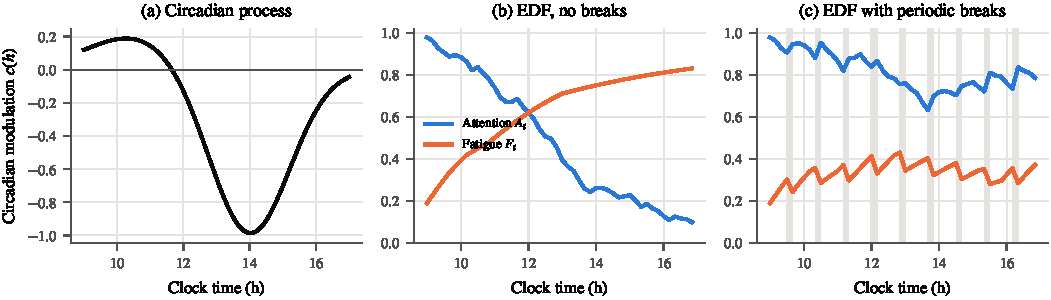
\includegraphics[width=\textwidth]{figures/fig_dynamics.pdf}
\caption{Simulator dynamics. (a) Circadian modulation $c(h)$ with a late-morning peak and post-lunch dip. (b) Effective attention and fatigue on one held-out test day under EDF without breaks. (c) The same day under EDF with a break after every four work slots (shaded bands mark breaks). Breaks keep attention high and fatigue low at the cost of working time.}
\label{fig:dynamics}
\end{figure}

\subsection{Observation model and partial observability}
The scheduler cannot observe $H_t$, $A_t$ or $F_t$. It receives noisy estimates
\begin{equation}
\tilde A_t=\mathrm{clip}(A_t+\sigma_o\epsilon^A_t,0,1),\qquad \tilde F_t=\mathrm{clip}(F_t+\sigma_o\epsilon^F_t,0,1),\qquad \epsilon^{A}_t,\epsilon^{F}_t\sim\mathcal N(0,1),
\label{eq:obs}
\end{equation}
with $\sigma_o=0.10$ in the nominal setting. These estimates stand in for wearable, ocular, behavioural or self-report estimators, whose errors are substantial in practice \cite{charles2019,borghini2014,hogervorst2014}. The full observation is the 13-dimensional vector
\begin{equation}
o_t=\Big[\tfrac{t}{T},\ \tilde A_t,\ \tilde F_t,\ \underbrace{\tfrac{n^e_t}{N},\ \tfrac{W^e_t}{20},\ \sigma^e_t,\ \tfrac{m^e_t}{N},\ \tfrac{\omega^e_t}{4}}_{\text{easy class}},\ \underbrace{\tfrac{n^h_t}{N},\ \tfrac{W^h_t}{20},\ \sigma^h_t,\ \tfrac{m^h_t}{N},\ \tfrac{\omega^h_t}{4}}_{\text{hard class}}\Big],
\label{eq:o}
\end{equation}
where, for each class, $n_t$ is the number of available unfinished tasks, $W_t$ their remaining work, $\sigma_t=\mathrm{clip}\big((\min_i D_i-t)/T,-1,1\big)$ the normalised slack of the most urgent task (1 if the class is empty), $m_t$ the number of overdue tasks, and $\omega_t$ the remaining work of the shortest task (0 if the class is empty). Unlike a binary completion vector, this summary is invariant to the number of tasks and exposes the deadline information that urgency-aware scheduling requires. The worker's true state and the future arrivals are hidden, so the decision problem is a POMDP $\langle\mathcal S,\mathcal A,P,R,\Omega,O,\gamma_{\mathrm{RL}}\rangle$ \cite{kaelbling1998}. Here $\mathcal S$ contains the full task set and $(H_t,F_t,t)$, $\Omega$ is the observation space of Eq.~\eqref{eq:o}, $O$ is given by Eq.~\eqref{eq:obs}, and $P$ by Eqs.~\eqref{eq:attention}--\eqref{eq:rho} together with the arrival process.

\subsection{Action space}
The agent chooses among five macro-actions,
\begin{equation}
\mathcal A=\{\textsc{easy},\ \textsc{hard},\ \textsc{edf},\ \textsc{spt},\ \textsc{break}\}.
\end{equation}
\textsc{easy} (\textsc{hard}) dispatches the available easy (hard) task with the earliest deadline, falling back to the other class if the chosen class is empty. \textsc{edf} and \textsc{spt} dispatch, across both classes, the task with the earliest deadline or the least remaining work. \textsc{break} allocates the slot to rest, and the worker also rests when no task is available. The first two actions let the agent regulate the cognitive \emph{intensity} of work relative to the worker's state. The two rule actions let it switch between urgency-driven and throughput-driven sequencing, in the spirit of DRL schedulers that select among dispatching rules \cite{luo2020,panzer2022}. This hybrid design has an important methodological consequence: every rule-based baseline in Section~\ref{sec:baselines} can be expressed as a policy over $\mathcal A$, so a learned policy is never handicapped relative to the baselines by its action space. Section~\ref{sec:component} reports an agent restricted to the intensity actions $\{\textsc{easy},\textsc{hard},\textsc{break}\}$ of the original formulation. The action space is independent of $N$, and tasks are preemptible at slot boundaries, which is common in knowledge work.

\subsection{Reward}
The per-slot reward combines task outcomes with cognitive terms:
\begin{equation}
r_t=\underbrace{\sum_{i\in\mathcal C_t}(1+d_i)\big[\mathbb 1(t+1\le D_i)+0.25\,\mathbb 1(t+1>D_i)\big]-0.5\,|\mathcal M_t|}_{r^{\text{task}}_t}\;+\;\mu A_{t+1}\;-\;\lambda F_{t+1},
\label{eq:reward}
\end{equation}
where $\mathcal C_t$ is the set of tasks completed in slot $t$, $\mathcal M_t$ is the set of tasks whose deadline expires unfinished at the end of slot $t$, $\mu=0.05$ and $\lambda=0.10$. Harder tasks are worth more, late completion retains a quarter of the value, and each missed deadline costs $0.5$. The attention and fatigue terms express the organisation's preference for sustainable work. Because such terms can change the optimal policy \cite{ng1999}, we (i) report reward-independent operational metrics (on-time rate, completion, fatigue exposure) alongside the return, (ii) train an agent with $\lambda=\mu=0$ to show that the learned behaviour is driven by the dynamics rather than by the reward terms, and (iii) sweep $\lambda$ to trace the productivity--fatigue Pareto front. The objective is to find a policy $\pi$ that maps observation histories to actions and maximises $\mathbb E_\pi\big[\sum_{t=0}^{T-1}\gamma_{\mathrm{RL}}^t r_t\big]$.

\begin{table}[t]
\centering
\caption{Nominal simulator parameters and their rationale.}
\label{tab:params}
\small
\begin{tabular}{p{4.3cm}lp{7.0cm}}
\toprule
Parameter & Value & Rationale / source \\
\midrule
Slots per day $T$, slot length $\Delta$ & 48, 10 min & 8-h workday; decision granularity of micro-breaks \cite{albulescu2022} \\
Tasks per day $N$ (initial / arriving) & 12 (6 / 6) & conditionally overloaded day; stochastic arrivals \\
Difficulty $d_i$, hard threshold & $\mathcal U[0.2,1]$, 0.6 & range of the original formulation \\
Work content $w_i$ & $1+2.5d_i$ units & 15--35 min at full capacity \\
Relative slack $s_i$ & $\mathcal U[0.3,1]$ & range of the original formulation \\
Attention depletion $\alpha$, fatigue coupling $\phi$ & 0.02, 0.5 & vigilance decrement over hours of work \cite{warm2008,thomson2015} \\
Attention recovery $\beta$ & 0.30 per slot & break benefits \cite{ariga2011,albulescu2022} \\
Circadian amplitude $\gamma$ & 0.15 & post-lunch dip \cite{monk2005,schmidt2007} \\
Fatigue accumulation $\delta$, recovery $\eta$ & 0.05, 0.20 & exponential fatigue--recovery \cite{jaber2010,jaber2013} \\
Fatigue throughput penalty $\kappa$ & 0.5 & performance loss under fatigue \cite{boksem2008,vandongen2003} \\
Process / observation noise $\sigma_p,\sigma_o$ & 0.02, 0.10 & variability; sensor error \cite{charles2019,hogervorst2014} \\
Reward weights $\mu,\lambda$ & 0.05, 0.10 & swept in Section~\ref{sec:pareto} \\
\bottomrule
\end{tabular}
\end{table}

\section{Attention-aware deep Q-network}\label{sec:method}

\subsection{From Q-learning to deep Q-networks}
For a fully observable MDP, the optimal action-value function satisfies the Bellman optimality equation
$Q^*(s,a)=\mathbb E\big[r+\gamma_{\mathrm{RL}}\max_{a'}Q^*(s',a')\,\big|\,s,a\big]$ \cite{puterman1994,sutton2018}, and tabular Q-learning converges to $Q^*$ under standard conditions \cite{watkins1992}. With continuous cognitive variables, a tabular representation is infeasible, so $Q$ is approximated by a neural network $Q(\cdot,\cdot;\theta)$ trained to minimise the temporal-difference (TD) error. The DQN of \citet{mnih2015} stabilises this nonlinear approximation with an experience replay buffer \cite{lin1992}, which breaks the temporal correlation of samples, and a periodically synchronised target network $\bar\theta$. Convergence is not guaranteed for nonlinear function approximation \cite{tsitsiklis1997}, so we assess stability empirically across independent seeds.

\subsection{Handling partial observability with an observation history}
In a POMDP, the optimal policy is a function of the belief $b_t(s)=\Pr(s_t=s\mid o_{0:t},a_{0:t-1})$ \cite{astrom1965,kaelbling1998}. Exact belief tracking is intractable for our continuous, nonlinear dynamics, and a memoryless policy $\pi(o_t)$ can be arbitrarily suboptimal \cite{singh1994}. Two structural properties of the scheduling problem make a short history informative. First, the latent state is persistent. $H_t$ and $F_t$ change slowly relative to the observation noise, so averaging several consecutive estimates reduces the error: for $k$ independent observations of a quasi-static quantity, the standard error falls by a factor $\sqrt k$. Second, the trajectory of the observations, for example fatigue rising after consecutive hard tasks or attention recovering after a break, reveals the direction and rate of change, which a single noisy reading cannot. We therefore feed the network the window
\begin{equation}
x_t=[o_{t-k+1},\dots,o_t]\in\mathbb R^{11k},\qquad k=4,
\end{equation}
zero-padded at the start of the day. This is the finite-memory approximation used for Atari \cite{mnih2015}. It is computationally cheaper than recurrent alternatives \cite{hausknecht2015,igl2018} and is a strong baseline for many POMDPs \cite{ni2022}. A 40-minute window spans the time scale of a typical work bout. Section~\ref{sec:component} varies $k\in\{1,2,4,8\}$.

\subsection{Double Q-learning and dueling architecture}
Max-based targets overestimate action values in noisy environments \cite{vanhasselt2016}, and our environment is noisy by design. AA-DQN therefore uses the Double-DQN target, which decouples action selection (online network) from evaluation (target network):
\begin{equation}
y_t=r_t+\gamma_{\mathrm{RL}}(1-\textit{done}_t)\,Q\big(x_{t+1},\ \arg\max_{a'}Q(x_{t+1},a';\theta);\ \bar\theta\big).
\label{eq:target}
\end{equation}
In many states, for example at the start of the day or when the queue is empty, the choice between easy and hard work matters much less than the value of the state itself. A dueling head \cite{wang2016dueling} represents this explicitly:
\begin{equation}
Q(x,a;\theta)=V(x;\theta)+\Big(A(x,a;\theta)-\tfrac1{|\mathcal A|}\textstyle\sum_{a'}A(x,a';\theta)\Big).
\end{equation}
The shared body consists of two fully connected layers of 128 ReLU units. The loss is the Huber loss of the TD error, which is robust to the occasional large reward of a hard task completed on time \cite{huber1964}:
\begin{equation}
\mathcal L(\theta)=\mathbb E_{(x,a,r,x')\sim\mathcal D}\big[\ell_{\delta=1}\big(Q(x,a;\theta)-y\big)\big].
\end{equation}
Parameters are updated with Adam \cite{kingma2015} and gradient-norm clipping. The vanilla DQN baseline differs from AA-DQN only in using $k=1$, the standard max target and a single linear output head. This isolates the contribution of memory and of the two stabilisation components.

\subsection{Exploration and training procedure}
Actions are selected $\epsilon$-greedily with an exponentially decaying exploration rate
$\epsilon_n=\epsilon_{\min}+(\epsilon_{\max}-\epsilon_{\min})e^{-\kappa_\epsilon n}$, where $n$ is the environment step, $\epsilon_{\max}=1$ and $\epsilon_{\min}=0.01$, and $\kappa_\epsilon$ is set so that $\epsilon$ reaches 0.05 after half of the training budget. Algorithm~\ref{alg:aadqn} summarises training. Every 100 episodes, the greedy policy is evaluated on a fixed set of 100 \emph{validation} days that are disjoint from the training and test days, and the parameters with the highest validation return are retained. This mirrors the tuning of the heuristic baselines on their own held-out days (Section~\ref{sec:baselines}), so that both families receive the same model-selection budget and neither sees the test days. For transparency we also report the final-iterate policy (Supplementary Table~S3).

\begin{algorithm}[t]
\caption{Training of the attention-aware DQN (AA-DQN).}
\label{alg:aadqn}
\small
\begin{algorithmic}[1]
\Require episodes $E$, history length $k$, replay capacity $|\mathcal D|$, batch size $B$, target period $C$, validation days $\mathcal V$
\State initialise $\theta$ randomly, $\bar\theta\gets\theta$, $\mathcal D\gets\emptyset$, $n\gets0$, $J^\star\gets-\infty$
\For{episode $e=1,\dots,E$}
  \State sample a workday (tasks, initial state, noise); observe $o_0$; $x_0\gets[\mathbf 0,\dots,\mathbf 0,o_0]$
  \For{$t=0,\dots,T-1$}
    \State $a_t\gets$ random action with prob.\ $\epsilon_n$, else $\arg\max_a Q(x_t,a;\theta)$
    \State dispatch $a_t$ (EDF within class or rest); simulate Eqs.~\eqref{eq:attention}--\eqref{eq:rho}; receive $r_t$ (Eq.~\eqref{eq:reward}) and $o_{t+1}$
    \State $x_{t+1}\gets$ shift$(x_t,o_{t+1})$; store $(x_t,a_t,r_t,x_{t+1},\textit{done}_t)$ in $\mathcal D$; $n\gets n+1$
    \If{$|\mathcal D|\ge$ warm-up}
      \State sample a minibatch of $B$ transitions; compute targets with Eq.~\eqref{eq:target}
      \State $\theta\gets\theta-\eta_{\mathrm{lr}}\,\mathrm{Adam}\big(\nabla_\theta\mathcal L(\theta)\big)$ with gradient clipping
    \EndIf
    \If{$n \bmod C=0$} $\bar\theta\gets\theta$ \EndIf
  \EndFor
  \If{$e \bmod 100=0$}
    \State $J\gets$ mean greedy return on $\mathcal V$; \textbf{if} $J>J^\star$ \textbf{then} $J^\star\gets J$, $\theta^\star\gets\theta$
  \EndIf
\EndFor
\State \Return $\theta^\star$
\end{algorithmic}
\end{algorithm}

\subsection{Computational complexity}
A forward pass costs $O(11k\cdot128+128^2+128\cdot|\mathcal A|)\approx2.3\times10^4$ multiply--accumulate operations, independent of the number of tasks, because the observation summarises the queue per class. The dispatch step is $O(N\log N)$. Inference therefore takes microseconds on a CPU (Section~\ref{sec:cost}), which is negligible relative to a 10-minute decision interval and allows deployment on wearable or edge devices.

\section{Experimental design}\label{sec:setup}

\subsection{Baselines}\label{sec:baselines}
We compare AA-DQN against the vanilla DQN and nine rule-based schedulers, which span classical dispatching and hand-crafted cognition-aware policies. Baselines dispatch individual tasks directly, so they have at least as much control over task choice as the RL agents.
\begin{itemize}
  \item \textbf{Random}: uniform choice among \textsc{easy}, \textsc{hard} and \textsc{break}.
  \item \textbf{FIFO}: the available task that arrived first; never rests.
  \item \textbf{EDF}: the available task with the earliest deadline; never rests \cite{jackson1955,liu1973}.
  \item \textbf{SPT}: the available task with the least remaining work; never rests \cite{smith1956}.
  \item \textbf{EDF-Periodic}: EDF with one break after every $p$ work slots, a fixed work--rest cycle in the spirit of ergonomic rest-allowance guidance \cite{konz1998}.
  \item \textbf{EDF-Threshold}: EDF that rests whenever the \emph{observed} fatigue exceeds $\tau_F$ or the observed attention falls below $\tau_A$. This is a reactive, state-aware rule.
  \item \textbf{SPT-Periodic} and \textbf{SPT-Threshold}: the same two rest rules combined with SPT sequencing. SPT limits the damage of overload by finishing short tasks first, so these variants combine the best classical sequencing rule (Section~\ref{sec:main}) with state-aware rest. They were added after a pre-submission review identified them as the strongest hand-designed competitors (Supplementary Section~S5).
  \item \textbf{Cog-Heuristic}: rests on the same threshold rule and otherwise schedules a hard task only when observed attention is at least $\tau_H$, an easy task otherwise (EDF within class). This hand-crafted rule encodes the intuition that the learned policy might discover.
\end{itemize}
The parameters of the five parametric heuristics were selected by exhaustive grid search, maximising mean return on 300 \emph{tuning} days that are disjoint from the training, validation and test days. The grids were $p\in\{2,3,4,5,6,8,10\}$; $\tau_F\in\{0.3,\dots,0.9,1.01\}$ and $\tau_A\in\{0,0.2,\dots,0.7\}$ (56 combinations, for both threshold rules); and, for Cog-Heuristic, $\tau_F\times\tau_A\times\tau_H$ with $\tau_H\in\{0.4,\dots,0.9\}$ (252 combinations). The heuristics observe exactly the same noisy signals as the agents. The selected parameters are reported in Supplementary Table~S2. Tuning is repeated separately for every environment variant, so that each ablation compares the agent with the best heuristic \emph{for that variant}.

\subsection{Protocol}
The main configurations were trained with ten independent seeds, the environment ablations and the domain-randomised variant with five, and the reward-weight sweep and the component study with three, each for 5000 episodes ($2.4\times10^5$ decisions). Four disjoint sets of days were used: training days (generated from the training seed), 100 validation days for checkpoint selection, 300 tuning days for heuristic parameters, and 500 test days used only once, for the final evaluation. All methods are evaluated greedily on the \emph{same} 500 test days with \emph{common random numbers}. Each test day fixes the task set, the initial cognitive state and the sequences of process and observation noise, so differences between methods are paired and not confounded by sampling variation. In total, 75 agents were trained and more than $10^5$ test days were simulated.

\subsection{Metrics}
Besides the return (Eq.~\eqref{eq:reward}), which depends on the reward weights, we report reward-independent operational metrics: the \emph{on-time rate} (fraction of the day's tasks completed by their deadline); the \emph{difficulty-weighted on-time rate} $\sum_i d_i\mathbb 1(\text{on time})/\sum_i d_i$; the \emph{completion rate} (completed at any time); the mean \emph{true} attention $\bar A$ and fatigue $\bar F$ over the day; the \emph{high-fatigue exposure}, i.e.\ the fraction of slots with $F_t>0.7$; and the \emph{break share}.

\subsection{Statistical analysis}
Following recommendations for reliable RL evaluation \cite{henderson2018,agarwal2021}, we treat the training seed as the unit of replication for learned policies. For each seed, metrics are averaged over the 500 test days. We report the mean and standard deviation across seeds, and 95\% bootstrap confidence intervals \cite{efron1979} with 5000 resamples. Deterministic heuristics are summarised across test days. To compare AA-DQN with each baseline, we average AA-DQN over seeds for each test day and apply the two-sided Wilcoxon signed-rank test \cite{wilcoxon1945} to the 500 paired day-level differences. We report the matched-pairs rank-biserial correlation $r_{rb}$ as effect size, the win rate, and Holm-adjusted $p$-values \cite{holm1979} over the nine baseline comparisons. As a more conservative seed-level check, we also report how many of the ten seeds outperform each baseline.

\subsection{Implementation}
The simulator, agents and baselines are implemented in Python with NumPy and PyTorch \cite{paszke2019}. Table~\ref{tab:hparams} lists the hyperparameters. Training used one CPU thread per run. The code, configuration files, raw per-day results and analysis scripts are released (see Data availability) so that every number and figure in this paper can be regenerated with a single command.

\begin{table}[t]
\centering
\caption{Agent hyperparameters (shared by DQN and AA-DQN unless stated).}
\label{tab:hparams}
\small
\begin{tabular}{lll}
\toprule
Hyperparameter & DQN & AA-DQN \\
\midrule
History length $k$ & 1 & 4 \\
Target & max (standard) & Double DQN \\
Output head & linear & dueling ($V$ + advantage) \\
Hidden layers & \multicolumn{2}{c}{2 $\times$ 128, ReLU} \\
Optimiser, learning rate & \multicolumn{2}{c}{Adam, $5\times10^{-4}$} \\
Discount $\gamma_{\mathrm{RL}}$ & \multicolumn{2}{c}{0.99} \\
Replay capacity, warm-up & \multicolumn{2}{c}{50\,000, 1\,000 transitions} \\
Minibatch size & \multicolumn{2}{c}{64} \\
Target update period $C$ & \multicolumn{2}{c}{1\,000 steps (hard copy)} \\
Loss, gradient clip & \multicolumn{2}{c}{Huber ($\delta=1$), $\|\nabla\|_2\le10$} \\
Exploration & \multicolumn{2}{c}{$\epsilon$: $1.0\rightarrow0.01$, exponential (0.05 at 50\% of budget)} \\
Action set & \multicolumn{2}{c}{\{\textsc{easy}, \textsc{hard}, \textsc{edf}, \textsc{spt}, \textsc{break}\}} \\
Training budget & \multicolumn{2}{c}{5\,000 episodes = 240\,000 decisions} \\
Checkpoint selection & \multicolumn{2}{c}{best greedy return on 100 validation days, every 100 episodes} \\
\bottomrule
\end{tabular}
\end{table}

\section{Results}\label{sec:results}

\subsection{Learning dynamics}
Figure~\ref{fig:curves} shows greedy validation performance during training, averaged over ten seeds. AA-DQN reaches the return of the best tuned heuristic after roughly 600 episodes, and the seed-averaged curve then fluctuates around that level. Its on-time rate, however, rises above the heuristic within 400 episodes and stays above it throughout. The seed average hides substantial checkpoint-to-checkpoint variation within each run. Individual checkpoints exceed the heuristic return by a clear margin, while others fall below it. This is the well-known policy oscillation of value-based deep RL under a constant learning rate \cite{henderson2018}, and it motivates selecting checkpoints on held-out validation days. Because validation and test days are disjoint, the test results in Section~\ref{sec:main} are not inflated by this selection. The vanilla DQN learns equally fast at first but stalls below the heuristic. Its \emph{training} return even declines after about 500 episodes (Supplementary Fig.~S2), as the exploration rate decreases and the memoryless agent increasingly commits to actions based on single noisy readings. This pattern is consistent with the over-estimation that Double Q-learning is designed to reduce \cite{vanhasselt2016} and with the known weakness of memoryless policies in POMDPs \cite{singh1994}. Validation-based selection picked checkpoints at episode \AADQNBestEp{} on average for AA-DQN and \DQNBestEp{} for DQN. The TD loss falls rapidly, rises moderately as value estimates grow, and then decreases slowly (Fig.~S2), the usual signature of bootstrapped value learning with a moving target.

\begin{figure}[t]
\centering
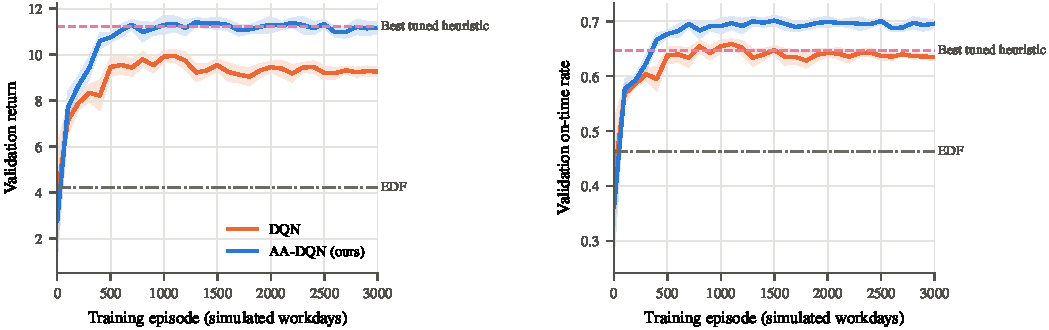
\includegraphics[width=\textwidth]{figures/fig_learning_curves.pdf}
\caption{Greedy validation performance during training (mean of ten seeds; shaded bands are 95\% confidence intervals). Horizontal lines show the best tuned heuristic (EDF-Periodic) and EDF on the same 100 validation days.}
\label{fig:curves}
\end{figure}

\subsection{Comparison with baselines}\label{sec:main}
Table~\ref{tab:main} and Fig.~\ref{fig:main} report performance on the 500 held-out test days. Three groups emerge. The rules that never rest (FIFO, EDF, SPT) drive the worker into the low-capacity regime: mean fatigue exceeds 0.47, attention falls to about 0.46--0.54, and EDF completes only \EDFOnTimePct\% of tasks on time. EDF performs particularly poorly, which is the overload domino effect known from real-time scheduling \cite{buttazzo2011}: once capacity falls, chasing the most urgent task means working on tasks that will be late anyway. SPT does better (\SPTOnTimePct\%) because finishing short tasks first limits the damage, but it still ignores the worker's state. The three cognition-aware heuristics, which rest about 19--20\% of the time, raise the on-time rate to 64--66\% and reduce mean fatigue by almost half. This confirms that the dynamics reward rest, as intended.

AA-DQN achieves the highest return (\aaReturn{}~$\pm$~\aaReturnSD) and the highest on-time rate (\aaOnTimePct\%) of all methods. Relative to the best tuned heuristic (\bestHeur), the paired difference is $+\dRetEDFPeriodic$ return (95\% CI [\dRetEDFPeriodicLo, \dRetEDFPeriodicHi]) and $+\dOnEDFPeriodic$ percentage points of on-time completion ([\dOnEDFPeriodicLo, \dOnEDFPeriodicHi]). Both are significant after Holm correction ($p<10^{-4}$; Table~\ref{tab:tests}). All ten seeds individually outperform every baseline. The effect sizes are medium for return ($r_{rb}=\rbRetEDFPeriodic$) and large for the on-time rate ($r_{rb}=\rbOnEDFPeriodic$). The day-to-day variability of all methods is large (standard deviation of about 3 return units across days), because some days are intrinsically harder than others. AA-DQN therefore does not win every day. It obtains a strictly higher return than \bestHeur{} on \winRetEDFPeriodicPct\% of days and a strictly higher on-time rate on \winOnEDFPeriodicPct\%, with ties on most of the remaining days. Relative to the vanilla DQN, adding memory and the two stabilisation components increases return by \dRetVsDqn{} ([\dRetVsDqnLo, \dRetVsDqnHi]) and wins on \winRetVsDqnPct\% of days.

Two qualifications place the gain in context. First, AA-DQN rests \emph{less} than the tuned heuristics (\AADQNBreakPct\% versus \bestHeurBreakPct\% of slots). It therefore operates at a somewhat higher mean fatigue (\aaFatigue{} versus \bestHeurFatigue). This level is still \fatigueRedVsEdfPct\% below EDF, and fatigue almost never exceeds 0.7 (high-fatigue exposure \AADQNHighFatPct\%, versus \EDFHighFatPct\% under EDF). Second, AA-DQN completes \emph{more tasks} on time while processing slightly \emph{less} total work than \bestHeur{}. Its difficulty-weighted on-time rate (\AADQNWOnTimePct\%) equals that of \bestHeur{} (\EDFPeriodicWOnTimePct\%). The improvement thus comes from \emph{which} tasks are worked on \emph{when}, not from extracting more effort from the worker. Section~\ref{sec:behaviour} analyses this behaviour.

Validation-based checkpoint selection matters for the size of the margin over the heuristics (Supplementary Table~S3). The final-iterate AA-DQN still completes more tasks on time than \bestHeur{} (\AADQNFinalOnTimePct\% versus \bestHeurOnTimePct\%) but its return (\AADQNFinalReturn) is on a par with the heuristic. The final-iterate vanilla DQN (\DQNFinalReturn) falls further behind. We report the validation-selected policy as the primary result because the heuristics received an equivalent selection step on their own held-out days.

\begin{table}[t]
\centering
\caption{Performance on 500 held-out test days (nominal environment). Learned policies: mean $\pm$ s.d.\ across ten training seeds of the per-seed test means. Heuristics: mean $\pm$ s.d.\ across test days (they are deterministic given the day). Bold marks the best value.}
\label{tab:main}
\small
\setlength{\tabcolsep}{3pt}
\resizebox{\textwidth}{!}{\begin{tabular}{lcccccc}
\toprule
Method & Return & On-time rate & Weighted on-time & Mean attention & Mean fatigue & Break share \\
\midrule
Random & 8.85 $\pm$ 2.71 & 0.535 $\pm$ 0.131 & 0.488 $\pm$ 0.143 & 0.855 $\pm$ 0.037 & 0.207 $\pm$ 0.045 & 0.326 $\pm$ 0.065 \\
FIFO & 3.49 $\pm$ 3.49 & 0.432 $\pm$ 0.139 & 0.422 $\pm$ 0.125 & 0.463 $\pm$ 0.106 & 0.546 $\pm$ 0.045 & 0.000 $\pm$ 0.003 \\
EDF & 4.24 $\pm$ 3.82 & 0.468 $\pm$ 0.155 & 0.454 $\pm$ 0.137 & 0.465 $\pm$ 0.105 & 0.545 $\pm$ 0.046 & 0.000 $\pm$ 0.003 \\
SPT & 7.95 $\pm$ 2.94 & 0.625 $\pm$ 0.120 & 0.494 $\pm$ 0.122 & 0.543 $\pm$ 0.093 & 0.477 $\pm$ 0.038 & 0.000 $\pm$ 0.001 \\
EDF-Periodic & 11.41 $\pm$ 3.32 & 0.660 $\pm$ 0.160 & 0.657 $\pm$ 0.148 & 0.798 $\pm$ 0.040 & 0.296 $\pm$ 0.029 & 0.188 $\pm$ 0.005 \\
EDF-Threshold & 11.35 $\pm$ 3.28 & 0.654 $\pm$ 0.164 & 0.650 $\pm$ 0.155 & 0.806 $\pm$ 0.022 & 0.288 $\pm$ 0.034 & 0.201 $\pm$ 0.037 \\
SPT-Periodic & 12.25 $\pm$ 2.04 & 0.709 $\pm$ 0.096 & 0.591 $\pm$ 0.111 & 0.817 $\pm$ 0.034 & 0.261 $\pm$ 0.023 & 0.188 $\pm$ 0.005 \\
SPT-Threshold & 12.30 $\pm$ 2.03 & 0.714 $\pm$ 0.099 & 0.597 $\pm$ 0.114 & 0.813 $\pm$ 0.022 & 0.268 $\pm$ 0.036 & 0.187 $\pm$ 0.035 \\
Cog-Heuristic & 10.59 $\pm$ 2.76 & 0.638 $\pm$ 0.132 & 0.533 $\pm$ 0.150 & 0.803 $\pm$ 0.034 & 0.279 $\pm$ 0.020 & 0.198 $\pm$ 0.025 \\
\midrule
DQN & 10.29 $\pm$ 0.26 & 0.677 $\pm$ 0.008 & 0.579 $\pm$ 0.012 & 0.677 $\pm$ 0.017 & 0.394 $\pm$ 0.018 & 0.108 $\pm$ 0.020 \\
AA-DQN (ours, primary) & 12.17 $\pm$ 0.15 & 0.728 $\pm$ 0.005 & 0.655 $\pm$ 0.012 & 0.754 $\pm$ 0.011 & 0.333 $\pm$ 0.012 & 0.150 $\pm$ 0.018 \\
AA-DQN, intensity actions (secondary) & \textbf{12.61 $\pm$ 0.18} & \textbf{0.740 $\pm$ 0.005} & \textbf{0.678 $\pm$ 0.008} & 0.770 $\pm$ 0.012 & 0.319 $\pm$ 0.014 & 0.162 $\pm$ 0.016 \\
\bottomrule
\end{tabular}}
\end{table}

\begin{figure}[t]
\centering
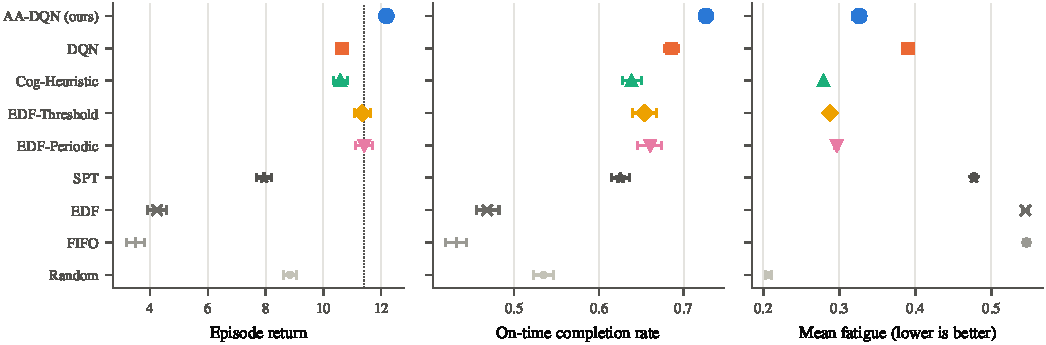
\includegraphics[width=\textwidth]{figures/fig_main_comparison.pdf}
\caption{Test performance with 95\% bootstrap confidence intervals (learned policies: across seeds; heuristics: across days). The dotted line marks the best heuristic return.}
\label{fig:main}
\end{figure}

\begin{table}[t]
\centering
\caption{Paired comparison of AA-DQN with each baseline on 500 common-random-number test days: mean difference with 95\% bootstrap CI, matched-pairs rank-biserial correlation $r_{rb}$, and Holm-adjusted Wilcoxon signed-rank $p$-values.}
\label{tab:tests}
\small
\resizebox{\textwidth}{!}{\begin{tabular}{lccccccccc}
\toprule
 & \multicolumn{3}{c}{Episode return} & \multicolumn{3}{c}{On-time rate (pp)} & \multicolumn{3}{c}{Weighted on-time rate (pp)} \\
\cmidrule(lr){2-4}\cmidrule(lr){5-7}\cmidrule(lr){8-10}
AA-DQN vs. & $\Delta$ [95\% CI] & $r_{rb}$ & $p_{\mathrm{Holm}}$ & $\Delta$ [95\% CI] & $r_{rb}$ & $p_{\mathrm{Holm}}$ & $\Delta$ [95\% CI] & $r_{rb}$ & $p_{\mathrm{Holm}}$ \\
\midrule
Random & +3.32 [+3.11, +3.52] & 0.97 & $<10^{-4}$ & +19.3 [+18.3, +20.3] & 1.00 & $<10^{-4}$ & +16.7 [+15.7, +17.7] & 0.98 & $<10^{-4}$ \\
FIFO & +8.68 [+8.46, +8.90] & 1.00 & $<10^{-4}$ & +29.6 [+28.7, +30.5] & 1.00 & $<10^{-4}$ & +23.3 [+22.5, +24.0] & 1.00 & $<10^{-4}$ \\
EDF & +7.93 [+7.70, +8.17] & 1.00 & $<10^{-4}$ & +26.0 [+25.0, +26.9] & 1.00 & $<10^{-4}$ & +20.0 [+19.3, +20.7] & 1.00 & $<10^{-4}$ \\
SPT & +4.22 [+4.05, +4.39] & 1.00 & $<10^{-4}$ & +10.2 [+9.6, +10.9] & 0.96 & $<10^{-4}$ & +16.1 [+15.3, +16.8] & 1.00 & $<10^{-4}$ \\
EDF-Periodic & +0.76 [+0.57, +0.94] & 0.34 & $<10^{-4}$ & +6.7 [+5.9, +7.6] & 0.69 & $<10^{-4}$ & -0.2 [-0.9, +0.5] & -0.05 & 0.6403 \\
EDF-Threshold & +0.82 [+0.64, +1.01] & 0.36 & $<10^{-4}$ & +7.4 [+6.6, +8.3] & 0.72 & $<10^{-4}$ & +0.5 [-0.2, +1.2] & 0.01 & 0.8269 \\
SPT-Periodic & -0.08 [-0.24, +0.08] & -0.06 & 0.2860 & +1.9 [+1.1, +2.6] & 0.24 & $<10^{-4}$ & +6.3 [+5.5, +7.2] & 0.62 & $<10^{-4}$ \\
SPT-Threshold & -0.13 [-0.29, +0.02] & -0.08 & 0.2390 & +1.4 [+0.7, +2.1] & 0.20 & 0.0002 & +5.7 [+4.9, +6.6] & 0.61 & $<10^{-4}$ \\
Cog-Heuristic & +1.58 [+1.43, +1.73] & 0.80 & $<10^{-4}$ & +8.9 [+8.3, +9.6] & 0.92 & $<10^{-4}$ & +12.2 [+11.4, +13.1] & 0.93 & $<10^{-4}$ \\
\bottomrule
\end{tabular}}
\end{table}


\section{Discussion}\label{sec:discussion}
\subsection{Ethical and organisational considerations}\label{sec:ethics}
A scheduler that monitors attention and fatigue and recommends when a person should work on what and when to rest touches on autonomy, privacy and fairness, and these issues must be designed in rather than added later \cite{parasuraman2000,feigh2012,amodei2016}. We see four requirements for responsible deployment. First, \emph{the system should be advisory}. Recommendations should be presented to the worker, who retains the authority to accept or override them; evidence from human--robot teaming indicates that the allocation of decision authority affects both efficiency and satisfaction \cite{gombolay2015}. Second, \emph{cognitive-state data are sensitive personal data}. Physiological and behavioural signals should be processed with informed consent, ideally on the worker's own device, and should never be used for performance appraisal. The observation model of AA-DQN needs only two scalar estimates per slot, which supports such data minimisation. Third, \emph{fairness across workers} requires that policies do not systematically disadvantage people whose fatigue dynamics differ from the nominal profile. Section~\ref{sec:robust} shows how performance changes for resilient and fatigue-prone profiles, and personalisation (Section~\ref{sec:future}) would further reduce such disparities. Fourth, \emph{safety constraints} should bound the policy, for example by guaranteeing a minimum amount of rest per period regardless of deadline pressure, consistent with safe RL principles \cite{garcia2015}. Notably, the learned policies in this study already increase rest relative to deadline-driven rules. The reward weight $\lambda$ makes the productivity--well-being trade-off explicit and auditable (Section~\ref{sec:pareto}), so stakeholders can choose it deliberately rather than leaving it implicit in a heuristic.

\subsection{Limitations}\label{sec:limitations}
The study has limitations that define its scope. (i) \emph{Simulation, not human data.} The cognitive model is grounded in established functional forms and its parameters were chosen to be behaviourally plausible, but it has not been calibrated against individual time-series of attention and fatigue. The absolute numbers should therefore be interpreted comparatively. The robustness analyses mitigate, but do not remove, this concern. (ii) \emph{Abstracted sensing.} Cognitive-state estimation is modelled as additive Gaussian noise on the true state. Real estimators can be biased, drift over the day, or fail intermittently, and they may be correlated with task type. (iii) \emph{A single worker and a single day.} Multi-day carry-over of fatigue, sleep, and team-level interactions such as hand-offs and shared deadlines are outside the scope. (iv) \emph{Action abstraction.} The agent chooses a difficulty class and delegates the choice of task within a class to EDF. This keeps the policy compact and size-invariant but excludes policies that, for example, deliberately abandon a hopeless task. (v) \emph{Algorithmic scope.} We study value-based agents with a finite history. Recurrent, model-based or policy-gradient agents \cite{hausknecht2015,igl2018,schulman2017} might extract more from the observation sequence. (vi) \emph{Simulated time-on-task effects only.} Motivation, task interest, interruptions and errors, which also shape real productivity \cite{mark2008,gonzalez2004,czerwinski2004}, are not modelled.

\subsection{Future work}\label{sec:future}
Three extensions follow directly. First, \emph{empirical calibration and validation}: fitting the latent dynamics to longitudinal data from vigilance probes, wearables and task logs \cite{basner2011,charles2019,shaffer2017}, then evaluating the scheduler in a controlled user study with NASA-TLX and performance outcomes \cite{hart1988}, ideally as a micro-randomised trial \cite{klasnja2015}. Second, \emph{personalisation}: domain randomisation over worker profiles during training \cite{tobin2017,zhao2020}, and Bayesian or meta-learning adaptation to an individual's parameters, in the spirit of personalised just-in-time interventions \cite{liao2020,nahumshani2018}. Third, \emph{multi-worker and human--robot settings}: extending the formulation to teams and to collaborative cells in which a robot absorbs demanding sub-tasks when a co-worker's attention is low \cite{ajoudani2018,lamon2019,zhang2022hrc,peternel2018}, with constrained or multi-objective RL to enforce explicit well-being guarantees \cite{hayes2022}.


\section{Conclusion}\label{sec:conclusion}
This paper formulated attention-aware task scheduling as a partially observable Markov decision process. In this formulation a worker's attention, fatigue and circadian state shape their capacity, rest is an explicit action, and the cognitive state is observed only through noisy estimates. We proposed a memory-augmented deep Q-network (AA-DQN) and evaluated it against nine rule-based schedulers, including grid-tuned EDF and SPT rules with periodic or state-triggered rest, using ten training seeds, 500 held-out workdays with common random numbers, and multiplicity-corrected tests.

Rules that ignore cognitive dynamics performed poorly, and every competitive policy rested in 15--20\% of the day. The pre-specified hybrid AA-DQN matched the return of the best tuned rule and achieved a higher on-time rate (\aaOnTimePct\% versus \bestHeurOnTimePct\%). A compact variant restricted to intensity actions, evaluated as a secondary analysis, exceeded the best rule in return (+\SecRetSPTThreshold), on-time rate (\AADQNThreeactOnTimePct\%) and difficulty-weighted on-time rate (\AADQNThreeactWOnTimePct\%). The learned policies are the only ones that combine high task throughput with protection of demanding tasks. They work intensively while the worker is fresh, schedule hard tasks when attention is high and rest around the post-lunch dip. Ablations showed that the value of learning grows sharply with the reliability of cognitive-state estimates, that memory is the critical architectural component, and that a moderate weight on fatigue improves both well-being and productivity.

The study is based on a behaviourally grounded but uncalibrated simulator. Its main limitation is therefore the gap to real workers, which future work will close through calibration with physiological and behavioural data, personalised policies, and user studies. The released simulator, agents and evaluation protocol provide a reproducible basis for that work and for fair comparisons of learned and hand-designed schedulers in human-centric systems.


\section*{CRediT authorship contribution statement}
\textbf{P.\,N. Bhargav Teja:} Conceptualization, Methodology, Software, Formal analysis, Investigation, Visualization, Writing -- original draft. \textbf{Lanka Sree Chathurya:} Methodology, Software, Validation, Data curation, Investigation, Writing -- original draft. \textbf{Rajay Vedaraj I.S.:} Conceptualization, Supervision, Methodology, Resources, Project administration, Writing -- review \& editing.

\section*{Declaration of competing interest}
The authors declare that they have no known competing financial interests or personal relationships that could have appeared to influence the work reported in this paper.

\section*{Funding}
This research did not receive any specific grant from funding agencies in the public, commercial, or not-for-profit sectors.

\section*{Data availability}
The simulator, agents, baselines, experiment configurations, raw per-episode results and the scripts that generate every table and figure are openly available at \url{https://github.com/bhargavteja-9779/rl}. No human-subject data were collected.

\section*{Declaration of generative AI and AI-assisted technologies in the manuscript preparation process}
During the preparation of this work the authors used an AI assistant (Claude, Anthropic) to support code development, language editing and the organisation of the manuscript. After using this tool, the authors reviewed and edited the content as needed and take full responsibility for the content of the published article.

\section*{Acknowledgements}
The authors thank Vellore Institute of Technology for providing the computational facilities used in this study.

\bibliographystyle{elsarticle-num}
\bibliography{references}

\end{document}
